\begin{appendix}

%------------------------------------------------------------------------------
\chapter{Oracle Data Types}\label{oracle-data-types}
%------------------------------------------------------------------------------
\index{Oracle Data Types}

\section*{Bind Data Types}\label{bind-data-types}

The \inline{oacdty} parameter in a bind variables details determines
the data type of that bind variable. This is not necessarily the data
type of the column in a table that it may be being \inline{INSERT}ed
or \inline{UPDATE}d into, or compared against.

The following data are taken from the \emph{Internal Data Types} section
of the \emph{Data Types} chapter in the 12cR2 
\href{http://docs.oracle.com/database/122/LNOCI/data-types.htm\#LNOCI16266}{\emph{Oracle Call
Interface} manual}.

Listed data types are:

\begin{longtable}[]{@{}r|l@{}}
\hline
\caption{Bind Variable data Types\ldots{}\textit{continues on next page}}
\endfoot
\caption{Bind Variable data Types}
\endlastfoot

\toprule
\begin{minipage}[b]{0.09\columnwidth}\raggedright\strut
Code\strut
\end{minipage} & \begin{minipage}[b]{0.43\columnwidth}\raggedright\strut
Data Type\strut
\end{minipage}\tabularnewline
\midrule
\endhead
\begin{minipage}[t]{0.09\columnwidth}\raggedright\strut
1\strut
\end{minipage} & \begin{minipage}[t]{0.43\columnwidth}\raggedright\strut
VARCHAR2 or NVARCHAR2\strut
\end{minipage}\tabularnewline
\begin{minipage}[t]{0.09\columnwidth}\raggedright\strut
2\strut
\end{minipage} & \begin{minipage}[t]{0.43\columnwidth}\raggedright\strut
NUMBER\strut
\end{minipage}\tabularnewline
\begin{minipage}[t]{0.09\columnwidth}\raggedright\strut
8\strut
\end{minipage} & \begin{minipage}[t]{0.43\columnwidth}\raggedright\strut
LONG\strut
\end{minipage}\tabularnewline
\begin{minipage}[t]{0.09\columnwidth}\raggedright\strut
11\strut
\end{minipage} & \begin{minipage}[t]{0.43\columnwidth}\raggedright\strut
ROWID\footnotemark{}\strut
\end{minipage}
\footnotetext{Code 11 is not officially listed by Oracle, but I have
  seen it in a trace file of my own for a ROWID data type.}\tabularnewline
\begin{minipage}[t]{0.09\columnwidth}\raggedright\strut
12\strut
\end{minipage} & \begin{minipage}[t]{0.43\columnwidth}\raggedright\strut
DATE\strut
\end{minipage}\tabularnewline
\begin{minipage}[t]{0.09\columnwidth}\raggedright\strut
23\strut
\end{minipage} & \begin{minipage}[t]{0.43\columnwidth}\raggedright\strut
RAW\strut
\end{minipage}\tabularnewline
\begin{minipage}[t]{0.09\columnwidth}\raggedright\strut
24\strut
\end{minipage} & \begin{minipage}[t]{0.43\columnwidth}\raggedright\strut
LONG RAW\strut
\end{minipage}\tabularnewline
\begin{minipage}[t]{0.09\columnwidth}\raggedright\strut
25\strut
\end{minipage} & \begin{minipage}[t]{0.43\columnwidth}\raggedright\strut
Unhandled data type\strut
\end{minipage}\tabularnewline
\begin{minipage}[t]{0.09\columnwidth}\raggedright\strut
29\strut
\end{minipage} & \begin{minipage}[t]{0.43\columnwidth}\raggedright\strut
Unhandled data type\strut
\end{minipage}\tabularnewline
\begin{minipage}[t]{0.09\columnwidth}\raggedright\strut
69\strut
\end{minipage} & \begin{minipage}[t]{0.43\columnwidth}\raggedright\strut
ROWID\strut
\end{minipage}\tabularnewline
\begin{minipage}[t]{0.09\columnwidth}\raggedright\strut
96\strut
\end{minipage} & \begin{minipage}[t]{0.43\columnwidth}\raggedright\strut
CHAR or NCHAR\strut
\end{minipage}\tabularnewline
\begin{minipage}[t]{0.09\columnwidth}\raggedright\strut
100\strut
\end{minipage} & \begin{minipage}[t]{0.43\columnwidth}\raggedright\strut
BINARY\_FLOAT\strut
\end{minipage}\tabularnewline
\begin{minipage}[t]{0.09\columnwidth}\raggedright\strut
101\strut
\end{minipage} & \begin{minipage}[t]{0.43\columnwidth}\raggedright\strut
BINARY\_DOUBLE\strut
\end{minipage}\tabularnewline
\begin{minipage}[t]{0.09\columnwidth}\raggedright\strut
102\strut
\end{minipage} & \begin{minipage}[t]{0.43\columnwidth}\raggedright\strut
REF\_CURSOR\footnotemark{}\strut
\end{minipage}
\footnotetext{Code 102 is not officially listed by Oracle, but I've seen
  REF CURSORs with this code in my own trace files.}\tabularnewline
\begin{minipage}[t]{0.09\columnwidth}\raggedright\strut
108\strut
\end{minipage} & \begin{minipage}[t]{0.43\columnwidth}\raggedright\strut
User-defined type -object type, VARRAY, nested table)\strut
\end{minipage}\tabularnewline
\begin{minipage}[t]{0.09\columnwidth}\raggedright\strut
111\strut
\end{minipage} & \begin{minipage}[t]{0.43\columnwidth}\raggedright\strut
REF\strut
\end{minipage}\tabularnewline
\begin{minipage}[t]{0.09\columnwidth}\raggedright\strut
112\strut
\end{minipage} & \begin{minipage}[t]{0.43\columnwidth}\raggedright\strut
CLOB or NCLOB\strut
\end{minipage}\tabularnewline
\begin{minipage}[t]{0.09\columnwidth}\raggedright\strut
113\strut
\end{minipage} & \begin{minipage}[t]{0.43\columnwidth}\raggedright\strut
BLOB\strut
\end{minipage}\tabularnewline
\begin{minipage}[t]{0.09\columnwidth}\raggedright\strut
114\strut
\end{minipage} & \begin{minipage}[t]{0.43\columnwidth}\raggedright\strut
BFILE\strut
\end{minipage}\tabularnewline
\begin{minipage}[t]{0.09\columnwidth}\raggedright\strut
123\strut
\end{minipage} & \begin{minipage}[t]{0.43\columnwidth}\raggedright\strut
VARRAY\footnotemark{}\strut
\end{minipage}
\footnotetext{Code 123 is not officially listed by Oracle, but I have
  seen it in a trace file of my own for a VARRAY data type.}\tabularnewline
\begin{minipage}[t]{0.09\columnwidth}\raggedright\strut
180\strut
\end{minipage} & \begin{minipage}[t]{0.43\columnwidth}\raggedright\strut
TIMESTAMP\strut
\end{minipage}\tabularnewline
\begin{minipage}[t]{0.09\columnwidth}\raggedright\strut
181\strut
\end{minipage} & \begin{minipage}[t]{0.43\columnwidth}\raggedright\strut
TIMESTAMP WITH TIME ZONE\strut
\end{minipage}\tabularnewline
\begin{minipage}[t]{0.09\columnwidth}\raggedright\strut
182\strut
\end{minipage} & \begin{minipage}[t]{0.43\columnwidth}\raggedright\strut
INTERVAL YEAR TO MONTH\strut
\end{minipage}\tabularnewline
\begin{minipage}[t]{0.09\columnwidth}\raggedright\strut
183\strut
\end{minipage} & \begin{minipage}[t]{0.43\columnwidth}\raggedright\strut
INTERVAL DAY TO SECOND\strut
\end{minipage}\tabularnewline
\begin{minipage}[t]{0.09\columnwidth}\raggedright\strut
208\strut
\end{minipage} & \begin{minipage}[t]{0.43\columnwidth}\raggedright\strut
UROWID\strut
\end{minipage}\tabularnewline
\begin{minipage}[t]{0.09\columnwidth}\raggedright\strut
231\strut
\end{minipage} & \begin{minipage}[t]{0.43\columnwidth}\raggedright\strut
TIMESTAMP WITH LOCAL TIME ZONE\strut
\end{minipage}\tabularnewline
\bottomrule
\end{longtable}

However, various other sources on the internet, and in books, seem to
disagree with some of what the above table shows. In addition, I have
come across at least one Oracle Trace where a ROWID was code 11 and not
code 69, also, I have seen VARRAY as code 123 and not as code 108.
Consistency? Who mentioned consistency?

%------------------------------------------------------------------------------
\chapter{Oracle Command Codes}\label{oracle-command-codes}
%------------------------------------------------------------------------------
\index{Oracle Command Codes}

\section*{Command Codes}\label{command-codes}

The \inline{oct} parameter in a \inline{PARSING IN CURSOR} line in an Oracle
trace file, determines the command that is being parsed in the SQL
statement. Why we should need this, I have no idea, as the SQL text for the
command will - obviously - show what command is being parsed. However\ldots{}

The following (large) table outlines the various command codes and was extracted
from an Oracle 12.1.0.2 database.

\begin{longtable}[]{@{}rl|rl|rl@{}}
\hline
\caption{Oracle Command Codes\ldots{}\textit{continues on next page}}
\endfoot
\caption{Oracle Command Codes}
\endlastfoot

\toprule
\begin{minipage}[b]{0.06\columnwidth}\raggedright\strut
Code\strut
\end{minipage} & \begin{minipage}[b]{0.19\columnwidth}\raggedright\strut
Command\strut
\end{minipage} & \begin{minipage}[b]{0.06\columnwidth}\raggedright\strut
Code\strut
\end{minipage} & \begin{minipage}[b]{0.24\columnwidth}\raggedright\strut
Command\strut
\end{minipage} & \begin{minipage}[b]{0.06\columnwidth}\raggedright\strut
Code\strut
\end{minipage} & \begin{minipage}[b]{0.24\columnwidth}\raggedright\strut
Command\strut
\end{minipage}\tabularnewline
\midrule
\endhead
\begin{minipage}[t]{0.06\columnwidth}\raggedright\strut
0\strut
\end{minipage} & \begin{minipage}[t]{0.19\columnwidth}\raggedright\strut
UNKNOWN\strut
\end{minipage} & \begin{minipage}[t]{0.06\columnwidth}\raggedright\strut
53\strut
\end{minipage} & \begin{minipage}[t]{0.24\columnwidth}\raggedright\strut
DROP USER\strut
\end{minipage} & \begin{minipage}[t]{0.06\columnwidth}\raggedright\strut
111\strut
\end{minipage} & \begin{minipage}[t]{0.24\columnwidth}\raggedright\strut
DROP PUBLIC SYNONYM\strut
\end{minipage}\tabularnewline
\begin{minipage}[t]{0.06\columnwidth}\raggedright\strut
1\strut
\end{minipage} & \begin{minipage}[t]{0.19\columnwidth}\raggedright\strut
CREATE TABLE\strut
\end{minipage} & \begin{minipage}[t]{0.06\columnwidth}\raggedright\strut
54\strut
\end{minipage} & \begin{minipage}[t]{0.24\columnwidth}\raggedright\strut
DROP ROLE\strut
\end{minipage} & \begin{minipage}[t]{0.06\columnwidth}\raggedright\strut
112\strut
\end{minipage} & \begin{minipage}[t]{0.24\columnwidth}\raggedright\strut
CREATE PUBLIC DATABASE LINK\strut
\end{minipage}\tabularnewline
\begin{minipage}[t]{0.06\columnwidth}\raggedright\strut
2\strut
\end{minipage} & \begin{minipage}[t]{0.19\columnwidth}\raggedright\strut
INSERT\strut
\end{minipage} & \begin{minipage}[t]{0.06\columnwidth}\raggedright\strut
55\strut
\end{minipage} & \begin{minipage}[t]{0.24\columnwidth}\raggedright\strut
SET ROLE\strut
\end{minipage} & \begin{minipage}[t]{0.06\columnwidth}\raggedright\strut
113\strut
\end{minipage} & \begin{minipage}[t]{0.24\columnwidth}\raggedright\strut
DROP PUBLIC DATABASE LINK\strut
\end{minipage}\tabularnewline
\begin{minipage}[t]{0.06\columnwidth}\raggedright\strut
3\strut
\end{minipage} & \begin{minipage}[t]{0.19\columnwidth}\raggedright\strut
SELECT\strut
\end{minipage} & \begin{minipage}[t]{0.06\columnwidth}\raggedright\strut
56\strut
\end{minipage} & \begin{minipage}[t]{0.24\columnwidth}\raggedright\strut
CREATE SCHEMA\strut
\end{minipage} & \begin{minipage}[t]{0.06\columnwidth}\raggedright\strut
114\strut
\end{minipage} & \begin{minipage}[t]{0.24\columnwidth}\raggedright\strut
GRANT ROLE\strut
\end{minipage}\tabularnewline
\begin{minipage}[t]{0.06\columnwidth}\raggedright\strut
4\strut
\end{minipage} & \begin{minipage}[t]{0.19\columnwidth}\raggedright\strut
CREATE CLUSTER\strut
\end{minipage} & \begin{minipage}[t]{0.06\columnwidth}\raggedright\strut
57\strut
\end{minipage} & \begin{minipage}[t]{0.24\columnwidth}\raggedright\strut
CREATE CONTROL FILE\strut
\end{minipage} & \begin{minipage}[t]{0.06\columnwidth}\raggedright\strut
115\strut
\end{minipage} & \begin{minipage}[t]{0.24\columnwidth}\raggedright\strut
REVOKE ROLE\strut
\end{minipage}\tabularnewline
\begin{minipage}[t]{0.06\columnwidth}\raggedright\strut
5\strut
\end{minipage} & \begin{minipage}[t]{0.19\columnwidth}\raggedright\strut
ALTER CLUSTER\strut
\end{minipage} & \begin{minipage}[t]{0.06\columnwidth}\raggedright\strut
59\strut
\end{minipage} & \begin{minipage}[t]{0.24\columnwidth}\raggedright\strut
CREATE TRIGGER\strut
\end{minipage} & \begin{minipage}[t]{0.06\columnwidth}\raggedright\strut
116\strut
\end{minipage} & \begin{minipage}[t]{0.24\columnwidth}\raggedright\strut
EXECUTE PROCEDURE\strut
\end{minipage}\tabularnewline
\begin{minipage}[t]{0.06\columnwidth}\raggedright\strut
6\strut
\end{minipage} & \begin{minipage}[t]{0.19\columnwidth}\raggedright\strut
UPDATE\strut
\end{minipage} & \begin{minipage}[t]{0.06\columnwidth}\raggedright\strut
60\strut
\end{minipage} & \begin{minipage}[t]{0.24\columnwidth}\raggedright\strut
ALTER TRIGGER\strut
\end{minipage} & \begin{minipage}[t]{0.06\columnwidth}\raggedright\strut
117\strut
\end{minipage} & \begin{minipage}[t]{0.24\columnwidth}\raggedright\strut
USER COMMENT\strut
\end{minipage}\tabularnewline
\begin{minipage}[t]{0.06\columnwidth}\raggedright\strut
7\strut
\end{minipage} & \begin{minipage}[t]{0.19\columnwidth}\raggedright\strut
DELETE\strut
\end{minipage} & \begin{minipage}[t]{0.06\columnwidth}\raggedright\strut
61\strut
\end{minipage} & \begin{minipage}[t]{0.24\columnwidth}\raggedright\strut
DROP TRIGGER\strut
\end{minipage} & \begin{minipage}[t]{0.06\columnwidth}\raggedright\strut
118\strut
\end{minipage} & \begin{minipage}[t]{0.24\columnwidth}\raggedright\strut
ENABLE TRIGGER\strut
\end{minipage}\tabularnewline
\begin{minipage}[t]{0.06\columnwidth}\raggedright\strut
8\strut
\end{minipage} & \begin{minipage}[t]{0.19\columnwidth}\raggedright\strut
DROP CLUSTER\strut
\end{minipage} & \begin{minipage}[t]{0.06\columnwidth}\raggedright\strut
62\strut
\end{minipage} & \begin{minipage}[t]{0.24\columnwidth}\raggedright\strut
ANALYZE TABLE\strut
\end{minipage} & \begin{minipage}[t]{0.06\columnwidth}\raggedright\strut
119\strut
\end{minipage} & \begin{minipage}[t]{0.24\columnwidth}\raggedright\strut
DISABLE TRIGGER\strut
\end{minipage}\tabularnewline
\begin{minipage}[t]{0.06\columnwidth}\raggedright\strut
9\strut
\end{minipage} & \begin{minipage}[t]{0.19\columnwidth}\raggedright\strut
CREATE INDEX\strut
\end{minipage} & \begin{minipage}[t]{0.06\columnwidth}\raggedright\strut
63\strut
\end{minipage} & \begin{minipage}[t]{0.24\columnwidth}\raggedright\strut
ANALYZE INDEX\strut
\end{minipage} & \begin{minipage}[t]{0.06\columnwidth}\raggedright\strut
120\strut
\end{minipage} & \begin{minipage}[t]{0.24\columnwidth}\raggedright\strut
ENABLE ALL TRIGGERS\strut
\end{minipage}\tabularnewline
\begin{minipage}[t]{0.06\columnwidth}\raggedright\strut
10\strut
\end{minipage} & \begin{minipage}[t]{0.19\columnwidth}\raggedright\strut
DROP INDEX\strut
\end{minipage} & \begin{minipage}[t]{0.06\columnwidth}\raggedright\strut
64\strut
\end{minipage} & \begin{minipage}[t]{0.24\columnwidth}\raggedright\strut
ANALYZE CLUSTER\strut
\end{minipage} & \begin{minipage}[t]{0.06\columnwidth}\raggedright\strut
121\strut
\end{minipage} & \begin{minipage}[t]{0.24\columnwidth}\raggedright\strut
DISABLE ALL TRIGGERS\strut
\end{minipage}\tabularnewline
\begin{minipage}[t]{0.06\columnwidth}\raggedright\strut
11\strut
\end{minipage} & \begin{minipage}[t]{0.19\columnwidth}\raggedright\strut
ALTER INDEX\strut
\end{minipage} & \begin{minipage}[t]{0.06\columnwidth}\raggedright\strut
65\strut
\end{minipage} & \begin{minipage}[t]{0.24\columnwidth}\raggedright\strut
CREATE PROFILE\strut
\end{minipage} & \begin{minipage}[t]{0.06\columnwidth}\raggedright\strut
122\strut
\end{minipage} & \begin{minipage}[t]{0.24\columnwidth}\raggedright\strut
NETWORK ERROR\strut
\end{minipage}\tabularnewline
\begin{minipage}[t]{0.06\columnwidth}\raggedright\strut
12\strut
\end{minipage} & \begin{minipage}[t]{0.19\columnwidth}\raggedright\strut
DROP TABLE\strut
\end{minipage} & \begin{minipage}[t]{0.06\columnwidth}\raggedright\strut
66\strut
\end{minipage} & \begin{minipage}[t]{0.24\columnwidth}\raggedright\strut
DROP PROFILE\strut
\end{minipage} & \begin{minipage}[t]{0.06\columnwidth}\raggedright\strut
123\strut
\end{minipage} & \begin{minipage}[t]{0.24\columnwidth}\raggedright\strut
EXECUTE TYPE\strut
\end{minipage}\tabularnewline
\begin{minipage}[t]{0.06\columnwidth}\raggedright\strut
13\strut
\end{minipage} & \begin{minipage}[t]{0.19\columnwidth}\raggedright\strut
CREATE SEQUENCE\strut
\end{minipage} & \begin{minipage}[t]{0.06\columnwidth}\raggedright\strut
67\strut
\end{minipage} & \begin{minipage}[t]{0.24\columnwidth}\raggedright\strut
ALTER PROFILE\strut
\end{minipage} & \begin{minipage}[t]{0.06\columnwidth}\raggedright\strut
128\strut
\end{minipage} & \begin{minipage}[t]{0.24\columnwidth}\raggedright\strut
FLASHBACK\strut
\end{minipage}\tabularnewline
\begin{minipage}[t]{0.06\columnwidth}\raggedright\strut
14\strut
\end{minipage} & \begin{minipage}[t]{0.19\columnwidth}\raggedright\strut
ALTER SEQUENCE\strut
\end{minipage} & \begin{minipage}[t]{0.06\columnwidth}\raggedright\strut
68\strut
\end{minipage} & \begin{minipage}[t]{0.24\columnwidth}\raggedright\strut
DROP PROCEDURE\strut
\end{minipage} & \begin{minipage}[t]{0.06\columnwidth}\raggedright\strut
129\strut
\end{minipage} & \begin{minipage}[t]{0.24\columnwidth}\raggedright\strut
CREATE SESSION\strut
\end{minipage}\tabularnewline
\begin{minipage}[t]{0.06\columnwidth}\raggedright\strut
15\strut
\end{minipage} & \begin{minipage}[t]{0.19\columnwidth}\raggedright\strut
ALTER TABLE\strut
\end{minipage} & \begin{minipage}[t]{0.06\columnwidth}\raggedright\strut
70\strut
\end{minipage} & \begin{minipage}[t]{0.24\columnwidth}\raggedright\strut
ALTER RESOURCE COST\strut
\end{minipage} & \begin{minipage}[t]{0.06\columnwidth}\raggedright\strut
130\strut
\end{minipage} & \begin{minipage}[t]{0.24\columnwidth}\raggedright\strut
ALTER MINING MODEL\strut
\end{minipage}\tabularnewline
\begin{minipage}[t]{0.06\columnwidth}\raggedright\strut
16\strut
\end{minipage} & \begin{minipage}[t]{0.19\columnwidth}\raggedright\strut
DROP SEQUENCE\strut
\end{minipage} & \begin{minipage}[t]{0.06\columnwidth}\raggedright\strut
71\strut
\end{minipage} & \begin{minipage}[t]{0.24\columnwidth}\raggedright\strut
CREATE MATERIALIZED VIEW LOG\strut
\end{minipage} & \begin{minipage}[t]{0.06\columnwidth}\raggedright\strut
131\strut
\end{minipage} & \begin{minipage}[t]{0.24\columnwidth}\raggedright\strut
SELECT MINING MODEL\strut
\end{minipage}\tabularnewline
\begin{minipage}[t]{0.06\columnwidth}\raggedright\strut
17\strut
\end{minipage} & \begin{minipage}[t]{0.19\columnwidth}\raggedright\strut
GRANT OBJECT\strut
\end{minipage} & \begin{minipage}[t]{0.06\columnwidth}\raggedright\strut
72\strut
\end{minipage} & \begin{minipage}[t]{0.24\columnwidth}\raggedright\strut
ALTER MATERIALIZED VIEW LOG\strut
\end{minipage} & \begin{minipage}[t]{0.06\columnwidth}\raggedright\strut
133\strut
\end{minipage} & \begin{minipage}[t]{0.24\columnwidth}\raggedright\strut
CREATE MINING MODEL\strut
\end{minipage}\tabularnewline
\begin{minipage}[t]{0.06\columnwidth}\raggedright\strut
18\strut
\end{minipage} & \begin{minipage}[t]{0.19\columnwidth}\raggedright\strut
REVOKE OBJECT\strut
\end{minipage} & \begin{minipage}[t]{0.06\columnwidth}\raggedright\strut
73\strut
\end{minipage} & \begin{minipage}[t]{0.24\columnwidth}\raggedright\strut
DROP MATERIALIZED VIEW LOG\strut
\end{minipage} & \begin{minipage}[t]{0.06\columnwidth}\raggedright\strut
134\strut
\end{minipage} & \begin{minipage}[t]{0.24\columnwidth}\raggedright\strut
ALTER PUBLIC SYNONYM\strut
\end{minipage}\tabularnewline
\begin{minipage}[t]{0.06\columnwidth}\raggedright\strut
19\strut
\end{minipage} & \begin{minipage}[t]{0.19\columnwidth}\raggedright\strut
CREATE SYNONYM\strut
\end{minipage} & \begin{minipage}[t]{0.06\columnwidth}\raggedright\strut
74\strut
\end{minipage} & \begin{minipage}[t]{0.24\columnwidth}\raggedright\strut
CREATE MATERIALIZED VIEW\strut
\end{minipage} & \begin{minipage}[t]{0.06\columnwidth}\raggedright\strut
135\strut
\end{minipage} & \begin{minipage}[t]{0.24\columnwidth}\raggedright\strut
DIRECTORY EXECUTE\strut
\end{minipage}\tabularnewline
\begin{minipage}[t]{0.06\columnwidth}\raggedright\strut
20\strut
\end{minipage} & \begin{minipage}[t]{0.19\columnwidth}\raggedright\strut
DROP SYNONYM\strut
\end{minipage} & \begin{minipage}[t]{0.06\columnwidth}\raggedright\strut
75\strut
\end{minipage} & \begin{minipage}[t]{0.24\columnwidth}\raggedright\strut
ALTER MATERIALIZED VIEW\strut
\end{minipage} & \begin{minipage}[t]{0.06\columnwidth}\raggedright\strut
136\strut
\end{minipage} & \begin{minipage}[t]{0.24\columnwidth}\raggedright\strut
SQL*LOADER DIRECT PATH LOAD\strut
\end{minipage}\tabularnewline
\begin{minipage}[t]{0.06\columnwidth}\raggedright\strut
21\strut
\end{minipage} & \begin{minipage}[t]{0.19\columnwidth}\raggedright\strut
CREATE VIEW\strut
\end{minipage} & \begin{minipage}[t]{0.06\columnwidth}\raggedright\strut
76\strut
\end{minipage} & \begin{minipage}[t]{0.24\columnwidth}\raggedright\strut
DROP MATERIALIZED VIEW\strut
\end{minipage} & \begin{minipage}[t]{0.06\columnwidth}\raggedright\strut
137\strut
\end{minipage} & \begin{minipage}[t]{0.24\columnwidth}\raggedright\strut
DATAPUMP DIRECT PATH UNLOAD\strut
\end{minipage}\tabularnewline
\begin{minipage}[t]{0.06\columnwidth}\raggedright\strut
22\strut
\end{minipage} & \begin{minipage}[t]{0.19\columnwidth}\raggedright\strut
DROP VIEW\strut
\end{minipage} & \begin{minipage}[t]{0.06\columnwidth}\raggedright\strut
77\strut
\end{minipage} & \begin{minipage}[t]{0.24\columnwidth}\raggedright\strut
CREATE TYPE\strut
\end{minipage} & \begin{minipage}[t]{0.06\columnwidth}\raggedright\strut
138\strut
\end{minipage} & \begin{minipage}[t]{0.24\columnwidth}\raggedright\strut
DATABASE STARTUP\strut
\end{minipage}\tabularnewline
\begin{minipage}[t]{0.06\columnwidth}\raggedright\strut
23\strut
\end{minipage} & \begin{minipage}[t]{0.19\columnwidth}\raggedright\strut
VALIDATE INDEX\strut
\end{minipage} & \begin{minipage}[t]{0.06\columnwidth}\raggedright\strut
78\strut
\end{minipage} & \begin{minipage}[t]{0.24\columnwidth}\raggedright\strut
DROP TYPE\strut
\end{minipage} & \begin{minipage}[t]{0.06\columnwidth}\raggedright\strut
139\strut
\end{minipage} & \begin{minipage}[t]{0.24\columnwidth}\raggedright\strut
DATABASE SHUTDOWN\strut
\end{minipage}\tabularnewline
\begin{minipage}[t]{0.06\columnwidth}\raggedright\strut
24\strut
\end{minipage} & \begin{minipage}[t]{0.19\columnwidth}\raggedright\strut
CREATE PROCEDURE\strut
\end{minipage} & \begin{minipage}[t]{0.06\columnwidth}\raggedright\strut
79\strut
\end{minipage} & \begin{minipage}[t]{0.24\columnwidth}\raggedright\strut
ALTER ROLE\strut
\end{minipage} & \begin{minipage}[t]{0.06\columnwidth}\raggedright\strut
140\strut
\end{minipage} & \begin{minipage}[t]{0.24\columnwidth}\raggedright\strut
CREATE SQL TXLN PROFILE\strut
\end{minipage}\tabularnewline
\begin{minipage}[t]{0.06\columnwidth}\raggedright\strut
25\strut
\end{minipage} & \begin{minipage}[t]{0.19\columnwidth}\raggedright\strut
ALTER PROCEDURE\strut
\end{minipage} & \begin{minipage}[t]{0.06\columnwidth}\raggedright\strut
80\strut
\end{minipage} & \begin{minipage}[t]{0.24\columnwidth}\raggedright\strut
ALTER TYPE\strut
\end{minipage} & \begin{minipage}[t]{0.06\columnwidth}\raggedright\strut
141\strut
\end{minipage} & \begin{minipage}[t]{0.24\columnwidth}\raggedright\strut
ALTER SQL TXLN PROFILE\strut
\end{minipage}\tabularnewline
\begin{minipage}[t]{0.06\columnwidth}\raggedright\strut
26\strut
\end{minipage} & \begin{minipage}[t]{0.19\columnwidth}\raggedright\strut
LOCK\strut
\end{minipage} & \begin{minipage}[t]{0.06\columnwidth}\raggedright\strut
81\strut
\end{minipage} & \begin{minipage}[t]{0.24\columnwidth}\raggedright\strut
CREATE TYPE BODY\strut
\end{minipage} & \begin{minipage}[t]{0.06\columnwidth}\raggedright\strut
142\strut
\end{minipage} & \begin{minipage}[t]{0.24\columnwidth}\raggedright\strut
USE SQL TXLN PROFILE\strut
\end{minipage}\tabularnewline
\begin{minipage}[t]{0.06\columnwidth}\raggedright\strut
27\strut
\end{minipage} & \begin{minipage}[t]{0.19\columnwidth}\raggedright\strut
NO-OP\strut
\end{minipage} & \begin{minipage}[t]{0.06\columnwidth}\raggedright\strut
82\strut
\end{minipage} & \begin{minipage}[t]{0.24\columnwidth}\raggedright\strut
ALTER TYPE BODY\strut
\end{minipage} & \begin{minipage}[t]{0.06\columnwidth}\raggedright\strut
143\strut
\end{minipage} & \begin{minipage}[t]{0.24\columnwidth}\raggedright\strut
DROP SQL TXLN PROFILE\strut
\end{minipage}\tabularnewline
\begin{minipage}[t]{0.06\columnwidth}\raggedright\strut
28\strut
\end{minipage} & \begin{minipage}[t]{0.19\columnwidth}\raggedright\strut
RENAME\strut
\end{minipage} & \begin{minipage}[t]{0.06\columnwidth}\raggedright\strut
83\strut
\end{minipage} & \begin{minipage}[t]{0.24\columnwidth}\raggedright\strut
DROP TYPE BODY\strut
\end{minipage} & \begin{minipage}[t]{0.06\columnwidth}\raggedright\strut
144\strut
\end{minipage} & \begin{minipage}[t]{0.24\columnwidth}\raggedright\strut
CREATE MEASURE FOLDER\strut
\end{minipage}\tabularnewline
\begin{minipage}[t]{0.06\columnwidth}\raggedright\strut
29\strut
\end{minipage} & \begin{minipage}[t]{0.19\columnwidth}\raggedright\strut
COMMENT\strut
\end{minipage} & \begin{minipage}[t]{0.06\columnwidth}\raggedright\strut
84\strut
\end{minipage} & \begin{minipage}[t]{0.24\columnwidth}\raggedright\strut
DROP LIBRARY\strut
\end{minipage} & \begin{minipage}[t]{0.06\columnwidth}\raggedright\strut
145\strut
\end{minipage} & \begin{minipage}[t]{0.24\columnwidth}\raggedright\strut
ALTER MEASURE FOLDER\strut
\end{minipage}\tabularnewline
\begin{minipage}[t]{0.06\columnwidth}\raggedright\strut
30\strut
\end{minipage} & \begin{minipage}[t]{0.19\columnwidth}\raggedright\strut
AUDIT OBJECT\strut
\end{minipage} & \begin{minipage}[t]{0.06\columnwidth}\raggedright\strut
85\strut
\end{minipage} & \begin{minipage}[t]{0.24\columnwidth}\raggedright\strut
TRUNCATE TABLE\strut
\end{minipage} & \begin{minipage}[t]{0.06\columnwidth}\raggedright\strut
146\strut
\end{minipage} & \begin{minipage}[t]{0.24\columnwidth}\raggedright\strut
DROP MEASURE FOLDER\strut
\end{minipage}\tabularnewline
\begin{minipage}[t]{0.06\columnwidth}\raggedright\strut
31\strut
\end{minipage} & \begin{minipage}[t]{0.19\columnwidth}\raggedright\strut
NOAUDIT OBJECT\strut
\end{minipage} & \begin{minipage}[t]{0.06\columnwidth}\raggedright\strut
86\strut
\end{minipage} & \begin{minipage}[t]{0.24\columnwidth}\raggedright\strut
TRUNCATE CLUSTER\strut
\end{minipage} & \begin{minipage}[t]{0.06\columnwidth}\raggedright\strut
147\strut
\end{minipage} & \begin{minipage}[t]{0.24\columnwidth}\raggedright\strut
CREATE CUBE BUILD PROCESS\strut
\end{minipage}\tabularnewline
\begin{minipage}[t]{0.06\columnwidth}\raggedright\strut
32\strut
\end{minipage} & \begin{minipage}[t]{0.19\columnwidth}\raggedright\strut
CREATE DATABASE LINK\strut
\end{minipage} & \begin{minipage}[t]{0.06\columnwidth}\raggedright\strut
88\strut
\end{minipage} & \begin{minipage}[t]{0.24\columnwidth}\raggedright\strut
ALTER VIEW\strut
\end{minipage} & \begin{minipage}[t]{0.06\columnwidth}\raggedright\strut
148\strut
\end{minipage} & \begin{minipage}[t]{0.24\columnwidth}\raggedright\strut
ALTER CUBE BUILD PROCESS\strut
\end{minipage}\tabularnewline
\begin{minipage}[t]{0.06\columnwidth}\raggedright\strut
33\strut
\end{minipage} & \begin{minipage}[t]{0.19\columnwidth}\raggedright\strut
DROP DATABASE LINK\strut
\end{minipage} & \begin{minipage}[t]{0.06\columnwidth}\raggedright\strut
91\strut
\end{minipage} & \begin{minipage}[t]{0.24\columnwidth}\raggedright\strut
CREATE FUNCTION\strut
\end{minipage} & \begin{minipage}[t]{0.06\columnwidth}\raggedright\strut
149\strut
\end{minipage} & \begin{minipage}[t]{0.24\columnwidth}\raggedright\strut
DROP CUBE BUILD PROCESS\strut
\end{minipage}\tabularnewline
\begin{minipage}[t]{0.06\columnwidth}\raggedright\strut
34\strut
\end{minipage} & \begin{minipage}[t]{0.19\columnwidth}\raggedright\strut
CREATE DATABASE\strut
\end{minipage} & \begin{minipage}[t]{0.06\columnwidth}\raggedright\strut
92\strut
\end{minipage} & \begin{minipage}[t]{0.24\columnwidth}\raggedright\strut
ALTER FUNCTION\strut
\end{minipage} & \begin{minipage}[t]{0.06\columnwidth}\raggedright\strut
150\strut
\end{minipage} & \begin{minipage}[t]{0.24\columnwidth}\raggedright\strut
CREATE CUBE\strut
\end{minipage}\tabularnewline
\begin{minipage}[t]{0.06\columnwidth}\raggedright\strut
35\strut
\end{minipage} & \begin{minipage}[t]{0.19\columnwidth}\raggedright\strut
ALTER DATABASE\strut
\end{minipage} & \begin{minipage}[t]{0.06\columnwidth}\raggedright\strut
93\strut
\end{minipage} & \begin{minipage}[t]{0.24\columnwidth}\raggedright\strut
DROP FUNCTION\strut
\end{minipage} & \begin{minipage}[t]{0.06\columnwidth}\raggedright\strut
151\strut
\end{minipage} & \begin{minipage}[t]{0.24\columnwidth}\raggedright\strut
ALTER CUBE\strut
\end{minipage}\tabularnewline
\begin{minipage}[t]{0.06\columnwidth}\raggedright\strut
36\strut
\end{minipage} & \begin{minipage}[t]{0.19\columnwidth}\raggedright\strut
CREATE ROLLBACK SEG\strut
\end{minipage} & \begin{minipage}[t]{0.06\columnwidth}\raggedright\strut
94\strut
\end{minipage} & \begin{minipage}[t]{0.24\columnwidth}\raggedright\strut
CREATE PACKAGE\strut
\end{minipage} & \begin{minipage}[t]{0.06\columnwidth}\raggedright\strut
152\strut
\end{minipage} & \begin{minipage}[t]{0.24\columnwidth}\raggedright\strut
DROP CUBE\strut
\end{minipage}\tabularnewline
\begin{minipage}[t]{0.06\columnwidth}\raggedright\strut
37\strut
\end{minipage} & \begin{minipage}[t]{0.19\columnwidth}\raggedright\strut
ALTER ROLLBACK SEG\strut
\end{minipage} & \begin{minipage}[t]{0.06\columnwidth}\raggedright\strut
95\strut
\end{minipage} & \begin{minipage}[t]{0.24\columnwidth}\raggedright\strut
ALTER PACKAGE\strut
\end{minipage} & \begin{minipage}[t]{0.06\columnwidth}\raggedright\strut
153\strut
\end{minipage} & \begin{minipage}[t]{0.24\columnwidth}\raggedright\strut
CREATE CUBE DIMENSION\strut
\end{minipage}\tabularnewline
\begin{minipage}[t]{0.06\columnwidth}\raggedright\strut
38\strut
\end{minipage} & \begin{minipage}[t]{0.19\columnwidth}\raggedright\strut
DROP ROLLBACK SEG\strut
\end{minipage} & \begin{minipage}[t]{0.06\columnwidth}\raggedright\strut
96\strut
\end{minipage} & \begin{minipage}[t]{0.24\columnwidth}\raggedright\strut
DROP PACKAGE\strut
\end{minipage} & \begin{minipage}[t]{0.06\columnwidth}\raggedright\strut
154\strut
\end{minipage} & \begin{minipage}[t]{0.24\columnwidth}\raggedright\strut
ALTER CUBE DIMENSION\strut
\end{minipage}\tabularnewline
\begin{minipage}[t]{0.06\columnwidth}\raggedright\strut
39\strut
\end{minipage} & \begin{minipage}[t]{0.19\columnwidth}\raggedright\strut
CREATE TABLESPACE\strut
\end{minipage} & \begin{minipage}[t]{0.06\columnwidth}\raggedright\strut
97\strut
\end{minipage} & \begin{minipage}[t]{0.24\columnwidth}\raggedright\strut
CREATE PACKAGE BODY\strut
\end{minipage} & \begin{minipage}[t]{0.06\columnwidth}\raggedright\strut
155\strut
\end{minipage} & \begin{minipage}[t]{0.24\columnwidth}\raggedright\strut
DROP CUBE DIMENSION\strut
\end{minipage}\tabularnewline
\begin{minipage}[t]{0.06\columnwidth}\raggedright\strut
40\strut
\end{minipage} & \begin{minipage}[t]{0.19\columnwidth}\raggedright\strut
ALTER TABLESPACE\strut
\end{minipage} & \begin{minipage}[t]{0.06\columnwidth}\raggedright\strut
98\strut
\end{minipage} & \begin{minipage}[t]{0.24\columnwidth}\raggedright\strut
ALTER PACKAGE BODY\strut
\end{minipage} & \begin{minipage}[t]{0.06\columnwidth}\raggedright\strut
157\strut
\end{minipage} & \begin{minipage}[t]{0.24\columnwidth}\raggedright\strut
CREATE DIRECTORY\strut
\end{minipage}\tabularnewline
\begin{minipage}[t]{0.06\columnwidth}\raggedright\strut
41\strut
\end{minipage} & \begin{minipage}[t]{0.19\columnwidth}\raggedright\strut
DROP TABLESPACE\strut
\end{minipage} & \begin{minipage}[t]{0.06\columnwidth}\raggedright\strut
99\strut
\end{minipage} & \begin{minipage}[t]{0.24\columnwidth}\raggedright\strut
DROP PACKAGE BODY\strut
\end{minipage} & \begin{minipage}[t]{0.06\columnwidth}\raggedright\strut
158\strut
\end{minipage} & \begin{minipage}[t]{0.24\columnwidth}\raggedright\strut
DROP DIRECTORY\strut
\end{minipage}\tabularnewline
\begin{minipage}[t]{0.06\columnwidth}\raggedright\strut
42\strut
\end{minipage} & \begin{minipage}[t]{0.19\columnwidth}\raggedright\strut
ALTER SESSION\strut
\end{minipage} & \begin{minipage}[t]{0.06\columnwidth}\raggedright\strut
100\strut
\end{minipage} & \begin{minipage}[t]{0.24\columnwidth}\raggedright\strut
LOGON\strut
\end{minipage} & \begin{minipage}[t]{0.06\columnwidth}\raggedright\strut
159\strut
\end{minipage} & \begin{minipage}[t]{0.24\columnwidth}\raggedright\strut
CREATE LIBRARY\strut
\end{minipage}\tabularnewline
\begin{minipage}[t]{0.06\columnwidth}\raggedright\strut
43\strut
\end{minipage} & \begin{minipage}[t]{0.19\columnwidth}\raggedright\strut
ALTER USER\strut
\end{minipage} & \begin{minipage}[t]{0.06\columnwidth}\raggedright\strut
101\strut
\end{minipage} & \begin{minipage}[t]{0.24\columnwidth}\raggedright\strut
LOGOFF\strut
\end{minipage} & \begin{minipage}[t]{0.06\columnwidth}\raggedright\strut
160\strut
\end{minipage} & \begin{minipage}[t]{0.24\columnwidth}\raggedright\strut
CREATE JAVA\strut
\end{minipage}\tabularnewline
\begin{minipage}[t]{0.06\columnwidth}\raggedright\strut
44\strut
\end{minipage} & \begin{minipage}[t]{0.19\columnwidth}\raggedright\strut
COMMIT\strut
\end{minipage} & \begin{minipage}[t]{0.06\columnwidth}\raggedright\strut
102\strut
\end{minipage} & \begin{minipage}[t]{0.24\columnwidth}\raggedright\strut
LOGOFF BY CLEANUP\strut
\end{minipage} & \begin{minipage}[t]{0.06\columnwidth}\raggedright\strut
161\strut
\end{minipage} & \begin{minipage}[t]{0.24\columnwidth}\raggedright\strut
ALTER JAVA\strut
\end{minipage}\tabularnewline
\begin{minipage}[t]{0.06\columnwidth}\raggedright\strut
45\strut
\end{minipage} & \begin{minipage}[t]{0.19\columnwidth}\raggedright\strut
ROLLBACK\strut
\end{minipage} & \begin{minipage}[t]{0.06\columnwidth}\raggedright\strut
103\strut
\end{minipage} & \begin{minipage}[t]{0.24\columnwidth}\raggedright\strut
SESSION REC\strut
\end{minipage} & \begin{minipage}[t]{0.06\columnwidth}\raggedright\strut
162\strut
\end{minipage} & \begin{minipage}[t]{0.24\columnwidth}\raggedright\strut
DROP JAVA\strut
\end{minipage}\tabularnewline
\begin{minipage}[t]{0.06\columnwidth}\raggedright\strut
46\strut
\end{minipage} & \begin{minipage}[t]{0.19\columnwidth}\raggedright\strut
SAVEPOINT\strut
\end{minipage} & \begin{minipage}[t]{0.06\columnwidth}\raggedright\strut
104\strut
\end{minipage} & \begin{minipage}[t]{0.24\columnwidth}\raggedright\strut
SYSTEM AUDIT\strut
\end{minipage} & \begin{minipage}[t]{0.06\columnwidth}\raggedright\strut
163\strut
\end{minipage} & \begin{minipage}[t]{0.24\columnwidth}\raggedright\strut
CREATE OPERATOR\strut
\end{minipage}\tabularnewline
\begin{minipage}[t]{0.06\columnwidth}\raggedright\strut
47\strut
\end{minipage} & \begin{minipage}[t]{0.19\columnwidth}\raggedright\strut
PL/SQL EXECUTE\strut
\end{minipage} & \begin{minipage}[t]{0.06\columnwidth}\raggedright\strut
105\strut
\end{minipage} & \begin{minipage}[t]{0.24\columnwidth}\raggedright\strut
SYSTEM NOAUDIT\strut
\end{minipage} & \begin{minipage}[t]{0.06\columnwidth}\raggedright\strut
164\strut
\end{minipage} & \begin{minipage}[t]{0.24\columnwidth}\raggedright\strut
CREATE INDEXTYPE\strut
\end{minipage}\tabularnewline
\begin{minipage}[t]{0.06\columnwidth}\raggedright\strut
48\strut
\end{minipage} & \begin{minipage}[t]{0.19\columnwidth}\raggedright\strut
SET TRANSACTION\strut
\end{minipage} & \begin{minipage}[t]{0.06\columnwidth}\raggedright\strut
106\strut
\end{minipage} & \begin{minipage}[t]{0.24\columnwidth}\raggedright\strut
AUDIT DEFAULT\strut
\end{minipage} & \begin{minipage}[t]{0.06\columnwidth}\raggedright\strut
165\strut
\end{minipage} & \begin{minipage}[t]{0.24\columnwidth}\raggedright\strut
DROP INDEXTYPE\strut
\end{minipage}\tabularnewline
\begin{minipage}[t]{0.06\columnwidth}\raggedright\strut
49\strut
\end{minipage} & \begin{minipage}[t]{0.19\columnwidth}\raggedright\strut
ALTER SYSTEM\strut
\end{minipage} & \begin{minipage}[t]{0.06\columnwidth}\raggedright\strut
107\strut
\end{minipage} & \begin{minipage}[t]{0.24\columnwidth}\raggedright\strut
NOAUDIT DEFAULT\strut
\end{minipage} & \begin{minipage}[t]{0.06\columnwidth}\raggedright\strut
166\strut
\end{minipage} & \begin{minipage}[t]{0.24\columnwidth}\raggedright\strut
ALTER INDEXTYPE\strut
\end{minipage}\tabularnewline
\begin{minipage}[t]{0.06\columnwidth}\raggedright\strut
50\strut
\end{minipage} & \begin{minipage}[t]{0.19\columnwidth}\raggedright\strut
EXPLAIN\strut
\end{minipage} & \begin{minipage}[t]{0.06\columnwidth}\raggedright\strut
108\strut
\end{minipage} & \begin{minipage}[t]{0.24\columnwidth}\raggedright\strut
SYSTEM GRANT\strut
\end{minipage} & \begin{minipage}[t]{0.06\columnwidth}\raggedright\strut
167\strut
\end{minipage} & \begin{minipage}[t]{0.24\columnwidth}\raggedright\strut
DROP OPERATOR\strut
\end{minipage}\tabularnewline
\begin{minipage}[t]{0.06\columnwidth}\raggedright\strut
51\strut
\end{minipage} & \begin{minipage}[t]{0.19\columnwidth}\raggedright\strut
CREATE USER\strut
\end{minipage} & \begin{minipage}[t]{0.06\columnwidth}\raggedright\strut
109\strut
\end{minipage} & \begin{minipage}[t]{0.24\columnwidth}\raggedright\strut
SYSTEM REVOKE\strut
\end{minipage} & \begin{minipage}[t]{0.06\columnwidth}\raggedright\strut
168\strut
\end{minipage} & \begin{minipage}[t]{0.24\columnwidth}\raggedright\strut
ASSOCIATE STATISTICS\strut
\end{minipage}\tabularnewline
\begin{minipage}[t]{0.06\columnwidth}\raggedright\strut
52\strut
\end{minipage} & \begin{minipage}[t]{0.19\columnwidth}\raggedright\strut
CREATE ROLE\strut
\end{minipage} & \begin{minipage}[t]{0.06\columnwidth}\raggedright\strut
110\strut
\end{minipage} & \begin{minipage}[t]{0.24\columnwidth}\raggedright\strut
CREATE PUBLIC SYNONYM\strut
\end{minipage} & \begin{minipage}[t]{0.06\columnwidth}\raggedright\strut
169\strut
\end{minipage} & \begin{minipage}[t]{0.24\columnwidth}\raggedright\strut
DISASSOCIATE STATISTICS\strut
\end{minipage}\tabularnewline
\begin{minipage}[t]{0.06\columnwidth}\raggedright\strut
170\strut
\end{minipage} & \begin{minipage}[t]{0.19\columnwidth}\raggedright\strut
CALL METHOD\strut
\end{minipage} & \begin{minipage}[t]{0.06\columnwidth}\raggedright\strut
199\strut
\end{minipage} & \begin{minipage}[t]{0.24\columnwidth}\raggedright\strut
PURGE TABLESPACE\strut
\end{minipage} & \begin{minipage}[t]{0.06\columnwidth}\raggedright\strut
218\strut
\end{minipage} & \begin{minipage}[t]{0.24\columnwidth}\raggedright\strut
CREATE FLASHBACK ARCHIVE\strut
\end{minipage}\tabularnewline
\begin{minipage}[t]{0.06\columnwidth}\raggedright\strut
171\strut
\end{minipage} & \begin{minipage}[t]{0.19\columnwidth}\raggedright\strut
CREATE SUMMARY\strut
\end{minipage} & \begin{minipage}[t]{0.06\columnwidth}\raggedright\strut
200\strut
\end{minipage} & \begin{minipage}[t]{0.24\columnwidth}\raggedright\strut
PURGE TABLE\strut
\end{minipage} & \begin{minipage}[t]{0.06\columnwidth}\raggedright\strut
219\strut
\end{minipage} & \begin{minipage}[t]{0.24\columnwidth}\raggedright\strut
ALTER FLASHBACK ARCHIVE\strut
\end{minipage}\tabularnewline
\begin{minipage}[t]{0.06\columnwidth}\raggedright\strut
172\strut
\end{minipage} & \begin{minipage}[t]{0.19\columnwidth}\raggedright\strut
ALTER SUMMARY\strut
\end{minipage} & \begin{minipage}[t]{0.06\columnwidth}\raggedright\strut
201\strut
\end{minipage} & \begin{minipage}[t]{0.24\columnwidth}\raggedright\strut
PURGE INDEX\strut
\end{minipage} & \begin{minipage}[t]{0.06\columnwidth}\raggedright\strut
220\strut
\end{minipage} & \begin{minipage}[t]{0.24\columnwidth}\raggedright\strut
DROP FLASHBACK ARCHIVE\strut
\end{minipage}\tabularnewline
\begin{minipage}[t]{0.06\columnwidth}\raggedright\strut
173\strut
\end{minipage} & \begin{minipage}[t]{0.19\columnwidth}\raggedright\strut
DROP SUMMARY\strut
\end{minipage} & \begin{minipage}[t]{0.06\columnwidth}\raggedright\strut
202\strut
\end{minipage} & \begin{minipage}[t]{0.24\columnwidth}\raggedright\strut
UNDROP OBJECT\strut
\end{minipage} & \begin{minipage}[t]{0.06\columnwidth}\raggedright\strut
225\strut
\end{minipage} & \begin{minipage}[t]{0.24\columnwidth}\raggedright\strut
ALTER DATABASE LINK\strut
\end{minipage}\tabularnewline
\begin{minipage}[t]{0.06\columnwidth}\raggedright\strut
174\strut
\end{minipage} & \begin{minipage}[t]{0.19\columnwidth}\raggedright\strut
CREATE DIMENSION\strut
\end{minipage} & \begin{minipage}[t]{0.06\columnwidth}\raggedright\strut
204\strut
\end{minipage} & \begin{minipage}[t]{0.24\columnwidth}\raggedright\strut
FLASHBACK DATABASE\strut
\end{minipage} & \begin{minipage}[t]{0.06\columnwidth}\raggedright\strut
226\strut
\end{minipage} & \begin{minipage}[t]{0.24\columnwidth}\raggedright\strut
CREATE PLUGGABLE DATABASE\strut
\end{minipage}\tabularnewline
\begin{minipage}[t]{0.06\columnwidth}\raggedright\strut
175\strut
\end{minipage} & \begin{minipage}[t]{0.19\columnwidth}\raggedright\strut
ALTER DIMENSION\strut
\end{minipage} & \begin{minipage}[t]{0.06\columnwidth}\raggedright\strut
205\strut
\end{minipage} & \begin{minipage}[t]{0.24\columnwidth}\raggedright\strut
FLASHBACK TABLE\strut
\end{minipage} & \begin{minipage}[t]{0.06\columnwidth}\raggedright\strut
227\strut
\end{minipage} & \begin{minipage}[t]{0.24\columnwidth}\raggedright\strut
ALTER PLUGGABLE DATABASE\strut
\end{minipage}\tabularnewline
\begin{minipage}[t]{0.06\columnwidth}\raggedright\strut
176\strut
\end{minipage} & \begin{minipage}[t]{0.19\columnwidth}\raggedright\strut
DROP DIMENSION\strut
\end{minipage} & \begin{minipage}[t]{0.06\columnwidth}\raggedright\strut
206\strut
\end{minipage} & \begin{minipage}[t]{0.24\columnwidth}\raggedright\strut
CREATE RESTORE POINT\strut
\end{minipage} & \begin{minipage}[t]{0.06\columnwidth}\raggedright\strut
228\strut
\end{minipage} & \begin{minipage}[t]{0.24\columnwidth}\raggedright\strut
DROP PLUGGABLE DATABASE\strut
\end{minipage}\tabularnewline
\begin{minipage}[t]{0.06\columnwidth}\raggedright\strut
177\strut
\end{minipage} & \begin{minipage}[t]{0.19\columnwidth}\raggedright\strut
CREATE CONTEXT\strut
\end{minipage} & \begin{minipage}[t]{0.06\columnwidth}\raggedright\strut
207\strut
\end{minipage} & \begin{minipage}[t]{0.24\columnwidth}\raggedright\strut
DROP RESTORE POINT\strut
\end{minipage} & \begin{minipage}[t]{0.06\columnwidth}\raggedright\strut
229\strut
\end{minipage} & \begin{minipage}[t]{0.24\columnwidth}\raggedright\strut
CREATE AUDIT POLICY\strut
\end{minipage}\tabularnewline
\begin{minipage}[t]{0.06\columnwidth}\raggedright\strut
178\strut
\end{minipage} & \begin{minipage}[t]{0.19\columnwidth}\raggedright\strut
DROP CONTEXT\strut
\end{minipage} & \begin{minipage}[t]{0.06\columnwidth}\raggedright\strut
208\strut
\end{minipage} & \begin{minipage}[t]{0.24\columnwidth}\raggedright\strut
PROXY AUTHENTICATION ONLY\strut
\end{minipage} & \begin{minipage}[t]{0.06\columnwidth}\raggedright\strut
230\strut
\end{minipage} & \begin{minipage}[t]{0.24\columnwidth}\raggedright\strut
ALTER AUDIT POLICY\strut
\end{minipage}\tabularnewline
\begin{minipage}[t]{0.06\columnwidth}\raggedright\strut
179\strut
\end{minipage} & \begin{minipage}[t]{0.19\columnwidth}\raggedright\strut
ALTER OUTLINE\strut
\end{minipage} & \begin{minipage}[t]{0.06\columnwidth}\raggedright\strut
209\strut
\end{minipage} & \begin{minipage}[t]{0.24\columnwidth}\raggedright\strut
DECLARE REWRITE EQUIVALENCE\strut
\end{minipage} & \begin{minipage}[t]{0.06\columnwidth}\raggedright\strut
231\strut
\end{minipage} & \begin{minipage}[t]{0.24\columnwidth}\raggedright\strut
DROP AUDIT POLICY\strut
\end{minipage}\tabularnewline
\begin{minipage}[t]{0.06\columnwidth}\raggedright\strut
180\strut
\end{minipage} & \begin{minipage}[t]{0.19\columnwidth}\raggedright\strut
CREATE OUTLINE\strut
\end{minipage} & \begin{minipage}[t]{0.06\columnwidth}\raggedright\strut
210\strut
\end{minipage} & \begin{minipage}[t]{0.24\columnwidth}\raggedright\strut
ALTER REWRITE EQUIVALENCE\strut
\end{minipage} & \begin{minipage}[t]{0.06\columnwidth}\raggedright\strut
232\strut
\end{minipage} & \begin{minipage}[t]{0.24\columnwidth}\raggedright\strut
CODE-BASED GRANT\strut
\end{minipage}\tabularnewline
\begin{minipage}[t]{0.06\columnwidth}\raggedright\strut
181\strut
\end{minipage} & \begin{minipage}[t]{0.19\columnwidth}\raggedright\strut
DROP OUTLINE\strut
\end{minipage} & \begin{minipage}[t]{0.06\columnwidth}\raggedright\strut
211\strut
\end{minipage} & \begin{minipage}[t]{0.24\columnwidth}\raggedright\strut
DROP REWRITE EQUIVALENCE\strut
\end{minipage} & \begin{minipage}[t]{0.06\columnwidth}\raggedright\strut
233\strut
\end{minipage} & \begin{minipage}[t]{0.24\columnwidth}\raggedright\strut
CODE-BASED REVOKE\strut
\end{minipage}\tabularnewline
\begin{minipage}[t]{0.06\columnwidth}\raggedright\strut
182\strut
\end{minipage} & \begin{minipage}[t]{0.19\columnwidth}\raggedright\strut
UPDATE INDEXES\strut
\end{minipage} & \begin{minipage}[t]{0.06\columnwidth}\raggedright\strut
212\strut
\end{minipage} & \begin{minipage}[t]{0.24\columnwidth}\raggedright\strut
CREATE EDITION\strut
\end{minipage} & \begin{minipage}[t]{0.06\columnwidth}\raggedright\strut
238\strut
\end{minipage} & \begin{minipage}[t]{0.24\columnwidth}\raggedright\strut
ADMINISTER KEY MANAGEMENT\strut
\end{minipage}\tabularnewline
\begin{minipage}[t]{0.06\columnwidth}\raggedright\strut
183\strut
\end{minipage} & \begin{minipage}[t]{0.19\columnwidth}\raggedright\strut
ALTER OPERATOR\strut
\end{minipage} & \begin{minipage}[t]{0.06\columnwidth}\raggedright\strut
213\strut
\end{minipage} & \begin{minipage}[t]{0.24\columnwidth}\raggedright\strut
ALTER EDITION\strut
\end{minipage} & \begin{minipage}[t]{0.06\columnwidth}\raggedright\strut
239\strut
\end{minipage} & \begin{minipage}[t]{0.24\columnwidth}\raggedright\strut
CREATE MATERIALIZED ZONEMAP\strut
\end{minipage}\tabularnewline
\begin{minipage}[t]{0.06\columnwidth}\raggedright\strut
190\strut
\end{minipage} & \begin{minipage}[t]{0.19\columnwidth}\raggedright\strut
PASSWORD CHANGE\strut
\end{minipage} & \begin{minipage}[t]{0.06\columnwidth}\raggedright\strut
214\strut
\end{minipage} & \begin{minipage}[t]{0.24\columnwidth}\raggedright\strut
DROP EDITION\strut
\end{minipage} & \begin{minipage}[t]{0.06\columnwidth}\raggedright\strut
240\strut
\end{minipage} & \begin{minipage}[t]{0.24\columnwidth}\raggedright\strut
ALTER MATERIALIZED ZONEMAP\strut
\end{minipage}\tabularnewline
\begin{minipage}[t]{0.06\columnwidth}\raggedright\strut
192\strut
\end{minipage} & \begin{minipage}[t]{0.19\columnwidth}\raggedright\strut
ALTER SYNONYM\strut
\end{minipage} & \begin{minipage}[t]{0.06\columnwidth}\raggedright\strut
215\strut
\end{minipage} & \begin{minipage}[t]{0.24\columnwidth}\raggedright\strut
DROP ASSEMBLY\strut
\end{minipage} & \begin{minipage}[t]{0.06\columnwidth}\raggedright\strut
241\strut
\end{minipage} & \begin{minipage}[t]{0.24\columnwidth}\raggedright\strut
DROP MATERIALIZED ZONEMAP\strut
\end{minipage}\tabularnewline
\begin{minipage}[t]{0.06\columnwidth}\raggedright\strut
197\strut
\end{minipage} & \begin{minipage}[t]{0.19\columnwidth}\raggedright\strut
PURGE USER\_RECYCLEBIN\strut
\end{minipage} & \begin{minipage}[t]{0.06\columnwidth}\raggedright\strut
216\strut
\end{minipage} & \begin{minipage}[t]{0.24\columnwidth}\raggedright\strut
CREATE ASSEMBLY\strut
\end{minipage} & \begin{minipage}[t]{0.06\columnwidth}\raggedright\strut
---\strut
\end{minipage} & \begin{minipage}[t]{0.24\columnwidth}\raggedright\strut
Lots Missing Here!\strut
\end{minipage}\tabularnewline
\begin{minipage}[t]{0.06\columnwidth}\raggedright\strut
198\strut
\end{minipage} & \begin{minipage}[t]{0.19\columnwidth}\raggedright\strut
PURGE DBA\_RECYCLEBIN\strut
\end{minipage} & \begin{minipage}[t]{0.06\columnwidth}\raggedright\strut
217\strut
\end{minipage} & \begin{minipage}[t]{0.24\columnwidth}\raggedright\strut
ALTER ASSEMBLY\strut
\end{minipage} & \begin{minipage}[t]{0.06\columnwidth}\raggedright\strut
305\strut
\end{minipage} & \begin{minipage}[t]{0.24\columnwidth}\raggedright\strut
ALTER PUBLIC DATABASE LINK\strut
\end{minipage}\tabularnewline
\bottomrule
\end{longtable}

The exact list of commands for your particular database version can be
extracted using the following SQL command:

\begin{lstlisting}[language=SQL]
select action as code,
       name as command
from   audit_action;
\end{lstlisting}

There are 212 different commands in Oracle 12c (12.1.0.2) while Oracle
11g (11.2.0.4) has only (!) 181.

%------------------------------------------------------------------------------
\chapter{Oracle Characterset Codes}\label{oracle-characterset-codes}
%------------------------------------------------------------------------------
\index{Oracle Characterset Codes}

\section*{Bind Charactersets}\label{bind-charactersets}

Some data types use different character sets. These are coded in the
\inline{csi} field in the bind details lines of the trace file.
Typical values that you may see here are as follows:

\begin{longtable}[]{@{}r|l@{}}
\toprule
\begin{minipage}[b]{0.09\columnwidth}\raggedright\strut
Code\strut
\end{minipage} & \begin{minipage}[b]{0.21\columnwidth}\raggedright\strut
Character Set\strut
\end{minipage}\tabularnewline
\midrule
\endhead
\hline
\caption{Bind Variable Character Sets}
\endfoot
\begin{minipage}[t]{0.09\columnwidth}\raggedright\strut
1\strut
\end{minipage} & \begin{minipage}[t]{0.21\columnwidth}\raggedright\strut
US7ASCII\strut
\end{minipage}\tabularnewline
\begin{minipage}[t]{0.09\columnwidth}\raggedright\strut
31\strut
\end{minipage} & \begin{minipage}[t]{0.21\columnwidth}\raggedright\strut
WE8ISO8859P1\strut
\end{minipage}\tabularnewline
\begin{minipage}[t]{0.09\columnwidth}\raggedright\strut
46\strut
\end{minipage} & \begin{minipage}[t]{0.21\columnwidth}\raggedright\strut
WE8ISO8859P15\strut
\end{minipage}\tabularnewline
\begin{minipage}[t]{0.09\columnwidth}\raggedright\strut
170\strut
\end{minipage} & \begin{minipage}[t]{0.21\columnwidth}\raggedright\strut
WE8MSWIN1250\strut
\end{minipage}\tabularnewline
\begin{minipage}[t]{0.09\columnwidth}\raggedright\strut
178\strut
\end{minipage} & \begin{minipage}[t]{0.21\columnwidth}\raggedright\strut
WE8MSWIN1252\strut
\end{minipage}\tabularnewline
\begin{minipage}[t]{0.09\columnwidth}\raggedright\strut
871\strut
\end{minipage} & \begin{minipage}[t]{0.21\columnwidth}\raggedright\strut
UTF8\strut
\end{minipage}\tabularnewline
\begin{minipage}[t]{0.09\columnwidth}\raggedright\strut
873\strut
\end{minipage} & \begin{minipage}[t]{0.21\columnwidth}\raggedright\strut
AL32UTF8\strut
\end{minipage}\tabularnewline
\begin{minipage}[t]{0.09\columnwidth}\raggedright\strut
2000\strut
\end{minipage} & \begin{minipage}[t]{0.21\columnwidth}\raggedright\strut
AL16UTF16\strut
\end{minipage}\tabularnewline
\bottomrule
\end{longtable}


%------------------------------------------------------------------------------
\chapter{How this Book Evolved}
%------------------------------------------------------------------------------
\label{how-this-book-evolved}%

\section{Why this Book?}\label{why-this-book}

This eBook originally started as a collection of useful notes, scripts, etc which I had come across, written or deduced, over the years of playing with Oracle Trace Files and various Trace File Analysis tools.

Eventually, I collected them all together in one place so that I could have all the useful information, in one easy to find place\footnote{I'm getting old, every day it seems. I am starting to forget things I knew - they are ageing out of the cache! I now appear to have the memory capacity of a small newt, so I need to have things written down!}.

There are many places on the internet, people I have met or worked with, books which I have bought (or had bought for me) and read, to whom I will always be grateful as they have taught me many things. Maybe I can help others as I have been helped.

As Isaac Newton\index{Newton, Isaac}\person{Newton, Isaac} is thought to have said, ``\emph{I have stood on the shoulders of giants}'' - me too.


\section{Creating the Book}\label{creating-the-book}

The book was created in plain text files, originally in \href{https://en.wikipedia.org/wiki/ReStructuredText}{ReStructuredText} mode, written (and edited) on both Windows\footnote{At work, in my lunch hour}, or on Linux - which I use for all my personal and business needs at home.

These RST files were simply a quick way to gather notes. They were then later enhanced by adding more detail and/or example code, and converted to \LaTeX{}\program{\LaTeX{}} by judicious use of the \href{https://pandoc.org/}{Pandoc}\program{Pandoc} text conversion utility, which I \emph{highly} recommend.

The converted \LaTeX{}\program{\LaTeX{}} files were then further enhanced, indexed, tidied up, etc using \href{http://www.texstudio.org/}{TexStudio}\program{TexStudio} which runs on both Windows and Linux, so I had the same development environment in both locations. Handy. 

The book itself, was created using a \LaTeX{}\program{\LaTeX{}} template called [the] \href{https://www.latextemplates.com/template/the-legrand-orange-book}{Legrand Orange Book Template} created by Mathias Legrand\index{Legrand, Mathias}. It is thanks to him that you get this book for free, because the licence terms of the book template specify no commercial use. I'm happy with that myself.

The front cover image on this book is taken from the book \emph{Kunstformen der Natur}\index{Kunstformen der Natur} by German biologist Ernst Haeckel\index{Haeckel, Ernst}\person{Haeckel, Ernst}. The book was published between 1899 and 1904. The image used is of various \emph{Discomedusae}\index{Discomedusae} which are a taxonomic group of jellyfish.

You can read about them on \href{https://en.wikipedia.org/wiki/Discomedusae}{Wikipedia} and there is a brief overview of the above book, also on \href{https://en.wikipedia.org/wiki/Kunstformen_der_Natur}{Wikipedia},
which shows a number of other images taken from the book. (Some of which I considered before choosing the current one!)

\emph{Discomedusae}\index{Discomedusae}\footnote{DiscoMedusae? Sounds like dancing jellyfish to me!} have absolutely nothing to do with Oracle or Trace Files - but I liked the image, and decided that it would make a good cover for the book and a decent enough chapter heading image too.

%------------------------------------------------------------------------------
\chapter{TraceAdjust Utility}
%------------------------------------------------------------------------------
\label{traceadjust}\program{TraceAdjust}

\section*{TraceAdjust Introduction}\label{traceadjust-introduction}


\emph{TraceAdjust} is a utility that I wrote to help me process the
myriads of trace files that I come across in my DBA work. You can get
the source code from github in my 
\href{https://github.com/NormanDunbar/TraceAdjust}{TraceAdjust repository} and compile it
on Windows or Linux/Unix with any decent C++ compiler.

It reads a normal trace file and writes out an adjusted one, as follows:

\begin{itemize}
\tightlist
\item
  The \inline{tim} values are converted to seconds, by inserting a
  decimal point in the appropriate position;
\item
  It adds a \inline{delta} to each \inline{tim} line. The delta is
  the number of microseconds between the \inline{tim} on this line,
  and the \inline{tim} on the previous (appropriate) trace line. This
  allows me to see how long passed between the previous \inline{tim}
  and this one. Occasionally useful.
\item
  It adds a \inline{dslt} to each \inline{tim} line. This is the
  ``delta since last timestamp'' and simply counts up the number of
  microseconds that have passed since the trace file last produced a
  timestamp line similar to the one in the header. Again, occasionally
  useful.
\item
  It adds a \inline{local} to each \inline{tim} line. This is a
  conversion of the \inline{tim} value on the line, to an actual
  date, in the current local timezone. The time part is resolved down to
  microsecond level. This is usually very useful!
\end{itemize}

Running a trace file through TraceAdjust\program{TraceAdjust} will create a new trace file,
which some trace analysing utilities cannot cope with due to the
additional fields that I have introduced. The Trace File Browser, in
Toad\program{Toad}, on the other hand, copes with my trace files quite happily and
simply ignores the additional data as appropriate.

%------------------------------------------------------------------------------
\chapter{TraceMiner2 Utility}
%------------------------------------------------------------------------------
\label{traceminer2-utility}
\program{TraceMiner2}

\section*{TraceMiner2 Introduction}\label{traceminer2-introduction}

So, you have a trace file, chock full of statements with lots of bind
variables in use. You \emph{need} to read through it to find out which
execution of any of the statements used which actual bind values. How is
this easily done?

\emph{TraceMiner2}\program{TraceMiner2}\footnote{There will be no more unashamed plugs in this
  document, I promise.} is another utility that I wrote to help me
process the myriads of trace files that I come across in my DBA work.

You can get the source code from github in my 
\href{https://github.com/NormanDunbar/TraceMiner2}{TraceMiner2 repository} and compile it
on Windows or Linux/Unix with any decent C++ compiler.

It reads a trace file and writes out an HTML report showing various
details of the SQL in the file, showing:

\begin{itemize}
\tightlist
\item
  The line number of the file where the SQL statement was found at
  (\inline{PARSING IN CURSOR});
\item
  The line number of the file where  the \inline{PARSE} statement was found at;
\item
  The line number of the file where  the \inline{BINDS} details were found at;
\item
  The line number of the file where  the \inline{EXEC} statement was found at;
\item
  The depth (\inline{dep}) of the statement when parsed etc.
\end{itemize}

You can choose to ignore statements over any given depth, so if you only
want top-level and \inline{dep=1} statements, just request \inline{--depth=1} on the
command line. 

The default HTML report appears as follows:

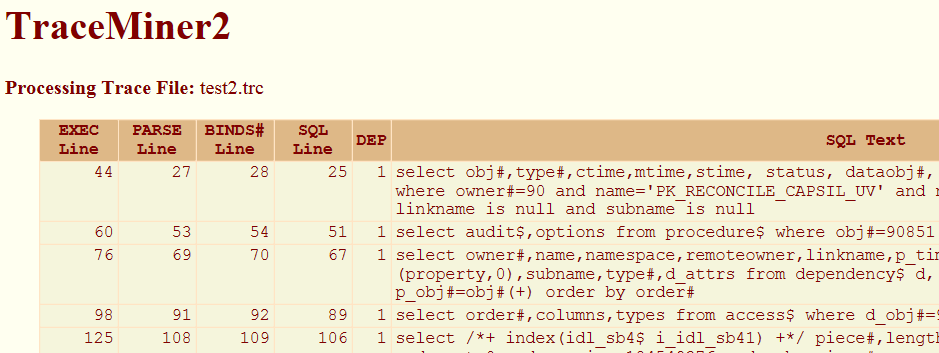
\includegraphics[width=\textwidth]{Content/images/TraceMiner2.png}

However, you can, if you have a standard report format at your company,
configure the generated css file to match that of your format.
\emph{TraceMiner2}\program{TraceMiner2} will not overwrite the css file if one exists in the
output folder.



\end{appendix}
